\section{Ecuaciones no lineales de segundo orden}

En este tema abordamos el estudio de las ecuaciones diferenciales ordinarias de segundo orden no lineales, centrándonos en dos modelos fundamentales con gran relevancia física y biológica: la \textbf{ecuación del péndulo} (con y sin rozamiento) y la \textbf{ecuación logística difusiva}. A través de estos modelos, analizaremos su formulación matemática, su reducción a sistemas autónomos de primer orden en el plano de fases, las propiedades de regularidad y carácter Lipschitziano (local frente a global), y la aplicación de los teoremas fundamentales de la teoría de Cauchy-Lipschitz para determinar la existencia global o la aparición de explosión en tiempo finito (\textit{blow-up}).

\subsection{La ecuación del péndulo}

Consideremos un péndulo simple formado por una masa puntual $m$ sujeta al extremo de una varilla inextensible y sin masa de longitud $\ell$, que oscila libremente en un plano vertical respecto a un punto de suspensión fijo.

La posición del péndulo queda unívocamente determinada en cada instante $t \in \mathbb{R}$ por el ángulo $u(t)$ (medido en radianes) que forma la varilla con la vertical descendente. La longitud de arco recorrida por la masa viene dada por:
\[
    s(t) = \ell \, u(t)
\]
Por tanto, la velocidad y aceleración tangenciales son, respectivamente, $s'(t) = \ell \, u'(t)$ y $s''(t) = \ell \, u''(t)$.

\begin{center}
\begin{tikzpicture}[scale=1.2, >=stealth]
    % Soporte superior (techo con rayado)
    \draw[thick] (-1.5, 0) -- (1.5, 0);
    \foreach \x in {-1.4,-1.1,...,1.3} {
        \draw[gray] (\x, 0) -- (\x+0.2, 0.25);
    }
    
    % Punto pivote fijo
    \coordinate (O) at (0, 0);
    \fill[black] (O) circle (2pt);
    
    % Parámetros geométricos del péndulo
    \def\L{3.6}       % Longitud de la varilla
    \def\ang{35}      % Ángulo con la vertical (grados)
    
    % Coordenada de la masa
    \coordinate (M) at ({\L*sin(\ang)}, {-\L*cos(\ang)});
    
    % Eje vertical de referencia
    \draw[dashed, gray!80!black] (0, 0) -- (0, -4.2);
    
    % Varilla del péndulo
    \draw[thick, black] (O) -- (M) node[midway, above right] {$\ell$};
    
    % Arco del ángulo u(t)
    \draw[->, thick, blue!80!black] (0, -1.2) arc (-90:{-90+\ang}:1.2);
    \node[blue!80!black] at (0.35, -1.5) {$u(t)$};
    
    % Arco de trayectoria circular s(t)
    \draw[dashed, red!70!black] (-25:{\L}) arc (-25:{-90-\ang+10}:{\L});
    \draw[->, thick, red!70!black] ({\L*sin(15)}, {-\L*cos(15)}) arc ({-90+15}:{-90+\ang}:{\L});
    \node[red!70!black, below right] at ({\L*sin(20)}, {-\L*cos(20)}) {$s(t) = \ell \, u(t)$};
    
    % Masa puntual m
    \draw[fill=blue!20, draw=blue!80!black, thick] (M) circle (0.28);
    \node at (M) {$m$};
    
    % Vectores de fuerzas
    % Peso P = m*g vertical hacia abajo
    \coordinate (Fg) at ($(M) + (0, -2.2)$);
    \draw[->, very thick, blue!80!black] (M) -- (Fg) node[below] {$\vec{P} = m\vec{g}$};
    
    % Componente normal F_N
    \coordinate (Fn) at ($(M) + ({2.2*cos(\ang)*sin(\ang)}, {-2.2*cos(\ang)*cos(\ang)})$);
    \draw[->, thick, cyan!80!black] (M) -- (Fn) node[below right] {$\vec{F}_N$};
    
    % Componente tangencial F_T (recuperadora)
    \coordinate (Ft) at ($(M) + ({-2.2*sin(\ang)*cos(\ang)}, {-2.2*sin(\ang)*sin(\ang)})$);
    \draw[->, very thick, cyan!80!black] (M) -- (Ft) node[left] {$\vec{F}_T$};
    
    % Líneas discontinuas del paralelogramo de fuerzas
    \draw[dashed, gray] (Ft) -- (Fg);
    \draw[dashed, gray] (Fn) -- (Fg);
    
    % Ángulo u(t) dentro del triángulo de fuerzas
    \draw[->, blue!80!black] ($(M) + (0, -0.9)$) arc (-90:{-90+\ang}:0.9);
    \node[blue!80!black, font=\footnotesize] at ($(M) + (0.2, -1.1)$) {$u(t)$};
    
    % Leyenda informativa
    \node[right, align=left, font=\small] at (1.8, -0.8) {
        $u(t)$: ángulo en radianes\\
        $s(t) = \ell \, u(t)$\\
        $\vec{F} = \vec{F}_N + \vec{F}_T$
    };
\end{tikzpicture}
\end{center}

Las fuerzas que actúan sobre la masa puntual son la tensión de la varilla (fuerza normal $\vec{F}_N$, dirigida en la dirección radial hacia el punto de suspensión) y la fuerza gravitatoria (peso $\vec{P} = m \vec{g}$ en dirección vertical descendente). Descomponiendo el peso en la dirección tangencial a la trayectoria obtenemos:
\[
    \sin u(t) = \frac{F_T}{m g} \implies F_T = - m g \sin u(t)
\]
donde el signo negativo refleja que se trata de una fuerza recuperadora, la cual actúa en sentido opuesto al desplazamiento angular.

Aplicando la segunda ley de Newton en la dirección tangencial:
\[
    F = m \, s''(t) = m \, \ell \, u''(t) = - m g \sin u(t)
\]
Dividiendo entre $m \ell$, obtenemos la \textbf{ecuación del péndulo libre}:
\[
    \boxed{u''(t) + \frac{g}{\ell} \sin u(t) = 0}
\]

\subsubsection{Péndulo con rozamiento del medio}

Si consideramos la presencia de fricción o rozamiento viscoso con el medio ambiente, se añade una fuerza resistente proporcional a la velocidad angular, con constante de amortiguamiento $r \geq 0$:
\[
    u''(t) + r u'(t) + \frac{g}{\ell} \sin u(t) = 0, \quad r \geq 0, \quad \frac{g}{\ell} > 0
\]

\subsubsection{Problema de valor inicial y formulación en el plano de fases}

El estado del péndulo queda completamente determinado al conocer el ángulo inicial $u_0$ y la velocidad angular inicial $v_0$ en un instante de tiempo $t_0 \in \mathbb{R}$. Planteamos así el problema de valor inicial:
\[
    (P) =
    \begin{cases}
        u'' + r u' + \frac{g}{\ell} \sin u = 0 \\
        u(t_0) = u_0, \quad u'(t_0) = v_0
    \end{cases}
\]

Para estudiar la existencia y unicidad de soluciones, reducimos esta ecuación escalar de segundo orden a un sistema equivalente de primer orden introduciendo las variables de estado:
\[
    u' = v, \quad v' = u'' = - r v - \frac{g}{\ell} \sin u
\]
En forma vectorial:
\[
    \begin{pmatrix} u \\ v \end{pmatrix}' =
    \begin{pmatrix} v \\ -r v - \frac{g}{\ell} \sin u \end{pmatrix} = f(u, v)
\]
donde el campo vectorial $f: \mathbb{R}^2 \to \mathbb{R}^2$ no depende explícitamente del tiempo $t$ (sistema autónomo) y es una función analítica ($\mathcal{C}^\infty$).

\subsubsection{Carácter Lipschitziano y existencia global}

Estudiemos las propiedades de regularidad de $f$. Calculemos su matriz jacobiana con respecto a las variables espaciales $(u, v)$:
\[
    D_{(u,v)} f(u, v) =
    \begin{pmatrix}
        0 & 1 \\
        -\frac{g}{\ell} \cos u & -r
    \end{pmatrix}
\]
Observemos que todas las entradas de la matriz jacobiana están acotadas uniformemente en todo $\mathbb{R}^2$:
\[
    \left| - \frac{g}{\ell} \cos u \right| \leq \frac{g}{\ell}, \quad |1| = 1, \quad |-r| = r
\]
Por consiguiente, el campo vectorial $f$ es \textbf{globalmente Lipschitziano} con respecto a $(u, v) \in \mathbb{R}^2$, uniformemente en $t \in \mathbb{R}$.

Aplicando el Teorema de Cauchy-Lipschitz global, para cada $n \geq 1$ el intervalo compacto $J_n = [t_0 - n, t_0 + n]$ admite una única solución $(u_n, v_n)$. Tomando límite:
\[
    (u, v) = \lim_{n \to \infty} (u_n, v_n)
\]
se obtiene la única solución global de $(P)$ en $t \in \mathbb{R}$, con intervalo maximal $I = (-\infty, +\infty)$.

\subsection{La ecuación logística difusiva}

En la década de 1930, se introdujeron modelos de reacción-difusión para estudiar la propagación espacial de genes ventajosos y dinámicas poblacionales donde los individuos se dispersan geográficamente.

Recordemos la ecuación logística clásica escalar, que modela el crecimiento con capacidad de carga en un ambiente homogéneo:
\[
    u' = \lambda u - a u^2, \quad \lambda, a > 0
\]
Si ahora los individuos están distribuidos espacialmente en una región $\Omega \subset \mathbb{R}^N$ y se desplazan aleatoriamente por difusión, la densidad de población $u(x, t)$ en la posición $x \in \Omega$ y en el tiempo $t > 0$ satisface la \textbf{ecuación logística difusiva}:
\[
    \frac{\partial u}{\partial t} - d \Delta u = \lambda u - a u^2
\]
donde:
\begin{itemize}
    \item $d > 0$ es el \textbf{coeficiente de difusión}.
    \item $-d \Delta u$ representa la \textbf{dispersión espacial} (término de difusión).
    \item $\Delta u = \sum_{i=1}^N \frac{\partial^2 u}{\partial x_i^2}$ es el operador Laplaciano en $\mathbb{R}^N$ (en $\mathbb{R}^3$, $\Delta u = \frac{\partial^2 u}{\partial x_1^2} + \frac{\partial^2 u}{\partial x_2^2} + \frac{\partial^2 u}{\partial x_3^2}$).
    \item $\lambda u - a u^2$ es el término cinético o de reacción biológica.
\end{itemize}

\begin{observación}
    El operador de difusión $\frac{\partial u}{\partial t} - d \Delta u = 0$ constituye la clásica ecuación del calor y la ley de transmisión por difusión:
    \begin{itemize}
        \item 1807: Jean-Baptiste Joseph Fourier (teoría analítica del calor).
        \item 1855: Adolf Fick (leyes de difusión en medios materiales).
        \item Década de 1930: Kolmogorov, Petrovsky, Piskunov y Ronald Fisher incorporan términos de reacción no lineales (ecuación KPP-Fisher).
    \end{itemize}
\end{observación}

\subsubsection{Condiciones de frontera y condiciones iniciales}

Consideremos un dominio acotado $\Omega \subset \mathbb{R}^N$ con frontera regular $\partial \Omega$.

\begin{center}
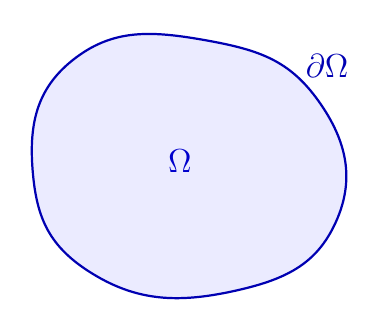
\begin{tikzpicture}[scale=1.1, >=stealth]
    % Dominio suave Omega
    \draw[thick, fill=blue!8, draw=blue!70!black] plot [smooth cycle, tension=0.8] coordinates {
        (-1.5, 0) (-1, 1.3) (0.5, 1.5) (1.8, 0.8) (2, -0.6) (0.8, -1.4) (-0.8, -1.2)
    };
    \node[blue!80!black, font=\large] at (0.2, 0.1) {$\Omega$};
    \node[blue!70!black, font=\large] at (1.9, 1.2) {$\partial \Omega$};
\end{tikzpicture}
\end{center}

Para determinar unívocamente la evolución del sistema, se especifican:
\begin{itemize}
    \item \textbf{Condición de frontera de Dirichlet homogénea:}
    \[
        u = 0 \text{ en } \partial \Omega, \quad \forall t > 0
    \]
    lo cual representa que la frontera del dominio es completamente inhóspita o letal para la población. Alternativamente, una condición de Neumann homogénea ($\frac{\partial u}{\partial n} = 0$ en $\partial \Omega$) representaría una frontera aislada o impenetrable.
    \item \textbf{Condición inicial:}
    \[
        u(x, t)\big|_{t = 0} = u_0(x), \quad x \in \Omega
    \]
\end{itemize}

El problema de contorno y de valor inicial conjunto toma la forma:
\[
    \begin{cases}
        \frac{\partial u}{\partial t} - d \Delta u = \lambda u - a u^2, & x \in \Omega, \quad t > 0 \\
        u = 0, & x \in \partial \Omega, \quad t > 0 \\
        u(x, 0) = u_0(x), & x \in \Omega
    \end{cases}
\]

\subsubsection{Estados de equilibrio (soluciones estacionarias)}

Los estados de equilibrio son soluciones independientes del tiempo, $u(x, t) \equiv u(x)$, en las cuales $\frac{\partial u}{\partial t} = 0$. Dichos equilibrios satisfacen el siguiente \textbf{problema de valores de contorno (PVC) elíptico}:
\[
    \begin{cases}
        -d \Delta u = \lambda u - a u^2 & \text{en } \Omega \\
        u = 0 & \text{en } \partial \Omega
    \end{cases}
\]

\subsubsection{Versión unidimensional}

En el caso unidimensional, el dominio espacial es un intervalo abierto $\Omega = (0, L) \subset \mathbb{R}$, con frontera $\partial \Omega = \{0, L\}$. El problema estacionario se reduce a una ecuación diferencial ordinaria de segundo orden:
\[
    -d u'' = \lambda u - a u^2 \implies -u'' = \frac{\lambda}{d} u - \frac{a}{d} u^2 = \tilde{\lambda} u - \tilde{a} u^2
\]
Reescalando los parámetros o normalizando $d = 1$, obtenemos la ecuación:
\[
    \boxed{-u'' = \lambda u - a u^2, \quad x \in (0, L) = \Omega}
\]
con condiciones de contorno de Dirichlet:
\[
    u(0) = u(L) = 0 \quad (u = 0 \text{ en } \partial \Omega)
\]
y ecuación de evolución temporal asociada:
\[
    \frac{\partial u}{\partial t} - \frac{\partial^2 u}{\partial x^2} = \lambda u - a u^2
\]

\subsection{Estudio del PVI para la ecuación logística de segundo orden}

Consideremos ahora la ecuación diferencial de segundo orden como un problema de valor inicial en una variable independiente temporal $t \in \mathbb{R}$:
\[
    \begin{cases}
        -u'' = \lambda u - a u^2, \quad \lambda, a \in \mathbb{R} \\
        u(t_0) = u_0, \quad u'(t_0) = v_0, \quad (u_0, v_0) \in \mathbb{R}^2
    \end{cases}
\]
Despejando la derivada de segundo orden:
\[
    u'' = a u^2 - \lambda u
\]

\subsubsection{Reducción a sistema de primer orden y carácter Lipschitz}

Definiendo la velocidad $u' = v$, transformamos el problema en un sistema plano de primer orden:
\[
    \begin{cases}
        u' = v \\
        v' = u'' = a u^2 - \lambda u
    \end{cases}
    \iff
    \begin{pmatrix} u \\ v \end{pmatrix}' =
    \begin{pmatrix} v \\ a u^2 - \lambda u \end{pmatrix} = f(u, v)
\]
con dato inicial $(u(t_0), v(t_0)) = (u_0, v_0)$, donde $v(t_0) = u'(t_0)$.

El campo vectorial $f: \mathbb{R}^2 \to \mathbb{R}^2$ es analítico, por lo que $f \in \mathcal{C}^\infty(\mathbb{R}^2, \mathbb{R}^2)$ y, en particular, $f$ es \textbf{localmente Lipschitziana} con respecto a $(u, v) \in \mathbb{R}^2$, uniformemente en $t \in \mathbb{R}$.

Calculemos su matriz jacobiana:
\[
    D_{(u,v)} f(u, v) =
    \begin{pmatrix}
        0 & 1 \\
        2 a u - \lambda & 0
    \end{pmatrix}
\]
Si $a \neq 0$, la entrada $2 a u - \lambda$ no está acotada cuando $|u| \to \infty$. En consecuencia:
\[
    f \text{ \textbf{no} puede ser globalmente Lipschitziana en } \mathbb{R}^2
\]
Por lo tanto, la teoría global no es aplicable y debemos limitarnos al marco de la \textbf{teoría local}.

\subsubsection{Comportamiento maximal: aplicación del Segundo Teorema Fundamental}

Al ser $f$ localmente Lipschitziana, el Teorema de existencia de soluciones maximales garantiza la existencia de una única solución maximal $(I, u, v) = (I, u, u')$ con intervalo maximal abierto:
\[
    I = (T_{\min}, T_{\max}), \quad -\infty \leq T_{\min} < t_0 < T_{\max} \leq +\infty
\]
Por el \textbf{Segundo Teorema Fundamental de Cauchy-Lipschitz}, sabemos que:
\begin{itemize}
    \item Hacia el futuro: si $T_{\max} < +\infty$, la solución explota en tiempo finito:
    \[
        \varlimsup_{t \nearrow T_{\max}} (|u(t)| + |u'(t)|) = +\infty
    \]
    \item Hacia el pasado: si $T_{\min} > -\infty$, la solución explota en tiempo finito hacia el pasado:
    \[
        \varlimsup_{t \searrow T_{\min}} (|u(t)| + |u'(t)|) = +\infty
    \]
\end{itemize}

\ejemplo{
    \textbf{Explosión en tiempo finito para el caso particular $a = 1, \lambda = 0$:}

    Consideremos el problema de valor inicial:
    \[
        \begin{cases}
            u'' = u^2 \\
            u(0) = x > 0 \\
            u'(0) = 0
        \end{cases}
    \]
    Por el teorema de Cauchy-Lipschitz local, existe una única solución maximal $(I, u)$ con intervalo maximal hacia el futuro $I = [0, T_{\max})$. Si $T_{\max} < +\infty$, el Segundo Teorema Fundamental asegura que:
    \[
        \lim_{t \nearrow T_{\max}} (|u(t)| + |u'(t)|) = +\infty
    \]

    \textbf{Demostración de que ocurre explosión en tiempo finito ($T_{\max} < +\infty$):}

    Multipliquemos ambos miembros de la ecuación por el factor integrante $u'(t)$:
    \[
        u'(t) u''(t) = u^2(t) u'(t) \implies \frac{d}{dt} \left[ \frac{1}{2} (u'(t))^2 \right] = \frac{d}{dt} \left[ \frac{1}{3} u^3(t) \right]
    \]
    Integrando entre $0$ y $t$:
    \[
        \frac{1}{2} (u'(t))^2 - \frac{1}{2} (u'(0))^2 = \frac{1}{3} u^3(t) - \frac{1}{3} u^3(0)
    \]
    Sustituyendo los datos iniciales $u(0) = x > 0$ y $u'(0) = 0$:
    \[
        (u'(t))^2 = \frac{2}{3} (u^3(t) - x^3)
    \]
    Como $u(0) = x > 0$ y $u''(0) = x^2 > 0$, la solución satisface $u'(t) > 0$ y $u(t) > x$ para todo $t > 0$. Tomando la raíz cuadrada positiva:
    \[
        u'(t) = \sqrt{\frac{2}{3}} \sqrt{u^3(t) - x^3}
    \]
    Separando variables e integrando entre $0$ y $t$:
    \[
        \int_x^{u(t)} \frac{du}{\sqrt{u^3 - x^3}} = \sqrt{\frac{2}{3}} t
    \]
    El tiempo máximo de existencia $T_{\max}$ viene determinado por el límite cuando $u \to +\infty$:
    \[
        T_{\max} = \sqrt{\frac{3}{2}} \int_x^{+\infty} \frac{du}{\sqrt{u^3 - x^3}}
    \]
    Efectuando el cambio de variable $u = x \, s$ (con $du = x \, ds$):
    \[
        T_{\max} = \sqrt{\frac{3}{2}} \int_1^{+\infty} \frac{x \, ds}{\sqrt{x^3 (s^3 - 1)}} = \sqrt{\frac{3}{2x}} \int_1^{+\infty} \frac{ds}{\sqrt{s^3 - 1}}
    \]
    Analicemos la convergencia de la integral impropia:
    \begin{itemize}
        \item Cerca de $s = 1$, factorizamos $s^3 - 1 = (s - 1)(s^2 + s + 1)$, por lo que $\frac{1}{\sqrt{s^3 - 1}} \sim \frac{1}{\sqrt{3}} (s - 1)^{-1/2}$, que es integrable en $[1, 2]$.
        \item Cuando $s \to +\infty$, $\frac{1}{\sqrt{s^3 - 1}} \sim s^{-3/2}$, y como el exponente es $3/2 > 1$, la integral converge en $[2, +\infty)$.
    \end{itemize}
    Por consiguiente, la integral converge a un valor estrictamente positivo y finito:
    \[
        T_{\max} = C \, x^{-1/2} < +\infty, \quad \text{con } C = \sqrt{\frac{3}{2}} \int_1^{+\infty} \frac{ds}{\sqrt{s^3 - 1}} > 0
    \]
    Esto demuestra de forma rigurosa que la solución maximal experimenta una explosión en tiempo finito (\textit{blow-up}) en $T_{\max} < +\infty$, con $\lim_{t \nearrow T_{\max}} u(t) = +\infty$.
}